
\documentclass[12pt]{beamer}
\mode<presentation>{\usetheme{Madrid}} % Either Madrid or Rochester

\usefonttheme{professionalfonts}
\usenavigationsymbolstemplate{}


\usepackage{graphicx}


\usepackage[utf8]{inputenc}
%\usepackage[T1]{fontenc}
\usepackage{palatino}
%\usepackage{euler}
%\usepackage{amsmath}
%\usepackage{amsthm}
%\usepackage{amssymb}
%\usepackage{amsthm,geometry}  
%\usepackage[colorlinks=true]{hyperref}

\newtheorem{cor}{Corollary}
\newtheorem{lem}{Lemma}
\newtheorem{thm}{Theorem}
\newtheorem{defin}{Definition}
\newtheorem{proposition}{Proposition}

%polices
\newcommand{\msf}{\mathsf}
\newcommand{\mrm}{\mathrm}
\newcommand{\mbf}{\mathbf}
\newcommand{\mbb}{\mathbb}
\newcommand{\mcal}{\mathcal}
%polices

\newcommand{\bra}[1]{\langle #1|}
\newcommand{\ket}[1]{|#1 \rangle}
\newcommand{\braket}[2]{\langle #1|#2\rangle}
\newcommand{\ketbra}[1]{\ket{#1}\bra{#1}}
\newcommand{\ketb}[2]{\ket{#1}\bra{#2}}
\newcommand{\ident}{\mathbb{I}}
\DeclareMathOperator{\tr}{\mathrm{Tr}}
\DeclareMathOperator{\rank}{rank}
\DeclareMathOperator{\polylog}{polylog}
\newcommand{\mdag}{^{\dag}} % dag operator
\newcommand{\demi}{\frac{1}{2}}

\newcommand{\state}{{\rho^{AE}}}
\newcommand{\mixed}{\frac{\mathbb{I}}{d_{A}} \otimes \rho^E}
\newcommand{\tra}{\tr_A}
\newcommand{\cypher}{\mathcal{E}}

\newcommand{\mpr}{{\mrm{Pr}}}
\newcommand{\mtr}[1]{\mathrm{Tr}\left(#1\right)}%trace
\newcommand{\mtra}[1]{\mathrm{Tr}_{A}\left(#1\right)}%trace
\newcommand{\mtrb}[1]{\mathrm{Tr}_{B}\left(#1\right)}%trace
\newcommand{\p}{^{\prime}}


%Nombres
\newcommand{\mbR}{\mathbb{R}}
\newcommand{\mbZ}{\mathbb{Z}}
\newcommand{\mbQ}{\mathbb{Q}}
\newcommand{\mbC}{\mathbb{C}}
\newcommand{\mbN}{\mathbb{N}}
\newcommand{\mbI}{\mathbb{I}}
\newcommand{\mE}[1]{\mcal{E}(#1)}
\newcommand{\mO}[1]{\mcal{O}(#1)}
\newcommand{\mbE}{\mathbb{E}}
%Nombres

%notation de circuit
\newcommand{\mh}{\mathrm{H}}
\newcommand{\mx}{\mathrm{X}}
\newcommand{\my}{\mathrm{Y}}
\newcommand{\mzz}{\mathrm{Z}}
\newcommand{\ms}{\mathrm{S}}
\newcommand{\mt}{\mathrm{T}}
\newcommand{\mamp}{\frac{1}{\sqrt{2}}}
\newcommand{\cnot}{\mathrm{CNOT}}
\newcommand{\msx}{\sigma_{x}}
\newcommand{\msy}{\sigma_{y}}
\newcommand{\msz}{\sigma_{z}}

%Des choses essentielles ˆ la beautŽ d'un papier
\setlength{\parindent}{0cm}
\setlength{\parskip}{2ex plus 0.5ex minus 0.5ex}

% Pour cette présentation
\newcommand{\aeq}{\approx_{(a)}}
\newcommand{\wtA}{\widetilde{A}}
\newcommand{\wtB}{\widetilde{B}}
\newcommand{\whA}{\widehat{A}}
\newcommand{\whB}{\widehat{B}}
\DeclareMathOperator{\Typ}{typ}

% ivan custom
\newcommand{\be}{\begin{equation}}
\newcommand{\ee}{\end{equation}}
\newcommand{\bea}{\begin{eqnarray}}
\newcommand{\eea}{\end{eqnarray}}
\newcommand{\e}{  \ensuremath{\mathcal E} }
\newcommand{\x}{  \ensuremath{\mathcal X} }
\newcommand{\y}{  \ensuremath{\mathcal Y} }
%\def \mcX{\mathcal{X} } (better no?)
\newcommand{\m}{  \ensuremath{\mathcal M} }
\newcommand{\otimesc}{\negthickspace\otimes\negthickspace}	%close verison of \otimes 
\newcommand{\typ}{  \ensuremath{ T^{(n)}_\epsilon  } }
\newcommand{\jtyp}{  \ensuremath{ A^{(n)}_\epsilon  } }
%%% THEOREMS   %%%%%%%%%%%%%%
\theoremstyle{plain}
\newtheorem{Th}{Theorem}[section]
\newtheorem{Lem}[Th]{Lemma}
\newtheorem{Prop}[Th]{Proposition}
\newtheorem{Cor}[Th]{Corollary}
\theoremstyle{definition}
\newtheorem{Ex}[Th]{Example}
\newtheorem{Def}[Th]{Definition}
\newtheorem{Rem}[Th]{Remark}
\newtheorem{Quest}[Th]{Question}
\newtheorem{prf}{Proof}
%%% MATH SETS %%%%%%%%%%%%%%
\def \Tr{\textup{Tr}}
\def \c{\mathbb{C}}
\def \z{\mathbb{Z}}
\def \r{\mathbb{R}}
\def \n{\mathbb{N}}
\def \p{\mathbb{P}}
\def \q{\mathbb{Q}}



\def\E{\mathcal{E}}
\def\cD{\mathcal{D}}
\def\cH{\mathcal{H}}
\def\cX{\mathcal{X}}
\def\cY{\mathcal{Y}}
\def\NN{\mathbb{N}}


% CAPACITY FORMULAS
\newcommand{\ICcap}{  \ensuremath{\mathcal C}_{IC} }
\newcommand{\MACcap}{  \ensuremath{\mathcal C}_{MAC} }
\newcommand{\MMACcap}{  \ensuremath{\mathcal C}_{MMAC} }
\newcommand{\Qcap}{  \ensuremath{\mathcal Q} }
\newcommand{\Ccap}{  \ensuremath{\mathcal C} }
\newcommand{\CcapEA}{  \ensuremath{\mathcal C}_{EA} }
\newcommand{\QcapEA}{  \ensuremath{\mathcal Q}_{EA} }






\title[IC \& quantum]{ Quantum interference channels }

\author[Ivan Savov]{Ivan Savov\\
McGill University\\
\strut\\
ECSE 612 Multiuser communications }
\date{April 16 2010}

\begin{document}

\begin{frame}
\titlepage
\end{frame}

%\begin{frame}
%	\frametitle{Outline}
%	\tableofcontent
%\end{frame}
%----------------------------------------------------------




\frame{
	\frametitle{Overview}
	\begin{enumerate}
		\item Definitions
		\item	Best bounds on the classical Interference Channel
		\item	Intro to Quantum Information Theory
		\item	Quantum MAC
		\item	Quantum Interference Channel
	\end{enumerate}

}


\frame{
	\frametitle{Definitions}
	
        \begin{definition}[Interference network]
            A two party interference network $(\cX_1 \otimes \cX_2, p(y_1,y_2|x_1,x_2), \cY_1 \otimes \cY_2)$ 
            is general model for communication networks with two inputs, two outputs and a probability transistion
            matrix $p(y_1,y_2|x_1,x_2)$.
        \end{definition}
        

        \begin{definition}[Interference channel]
            A two party interference channel is a particular use of an interference network 
            $(\cX_1 \otimes \cX_2, p(y_1,y_2|x_1,x_2), \cY_1 \otimes \cY_2)$ 
            where messages $M_1,M_2$ are independently encoded into a codewords $X_1,X_2$ 
            at rates $(R_1,R_2)$ with $Y_1,Y_2$ being the intended receiver.
        \end{definition}
}



\frame{
	\frametitle{Best inner bound}
	
	{\bf Han Kobayashi / Cheng Motani Garg inner bound}
        \be	% don't need \operatorname{conv} since we have Q
        		G_{HK}  = G_{CMG} =  \cup_{p(x_1|u_1)p(x_2|u_2)p(u_1)p(u_2)} \{ (R_1,R_2) | \text{ Eqn. \eqref{Rcmg} } \}  \nonumber
        \ee
	\bea
		R_1 		&\leq&	I(X_1;Y_1| U_2 Q) \nonumber \\
		R_2 		&\leq&	I(X_2;Y_2| U_1 Q) \nonumber \\
	R_1 + R_2	&\leq&	I(X_1U_2; Y_1|Q) + I (X_2; Y_2|U_1U_2Q) \nonumber \\
	R_1 + R_2	&\leq&	I (X_1; Y_1|U_1U_2Q) + I (X_2U_1; Y_2|Q) \label{Rcmg}\\
	R_1 + R_2	&\leq&	I (X_1U_2; Y_1|U_1Q) + I(X_2U_1; Y_2|U_2Q) \nonumber  \\
	2R_1 + R_2	&\leq&	I (X_1U_2; Y_1|Q) + I (X_1; Y_1|U_1U_2Q) + I(X_2U_1;Y_2|U_2Q) \nonumber \\
	R_1 + 2R_2	&\leq&	I (X_2; Y_2|U_1U_2Q) + I (X_2U_1; Y_2|Q) +  I (X_1U_2; Y_1|U_1Q) \nonumber 
	\eea
}

\frame{
	\frametitle{First outer bound}
         \be
        		G_{Naive}  \triangleq \operatorname{conv} \cup_{p(x_1)p(x_2)} \{ (R_1,R_2) | \text{ Eqn. \eqref{Gnaive} } \} 
        \ee
        \bea \label{eqn:naive-bound}
            R_1     &\leq&    I(X_1;Y_2|X_2) \nonumber \\
            R_2     &\leq&    I(X_2;Y_2|X_1) \label{Gnaive}
        \eea
        
        %Claim:  $\ICcap \subset G_{Naive}$. \\

}


\frame{
	\frametitle{Sato outer bound}
        \be
        		G_{Sato}  \triangleq \operatorname{conv} \cup_{p(x_1)p(x_2)} \{ (R_1,R_2) | \text{ Eqn. \eqref{Gsato} } \} 
        \ee
        \bea \label{eqn:sato-outer-bound}
            R_1             &\leq&    I(X_1;Y_2|X_2)  \nonumber \\
            R_2             &\leq&    I(X_2;Y_2|X_1)  \label{Gsato} \\
            R_1+R_2    &\leq&    I(X_1X_2;Y_1Y_2) \nonumber 
        \eea
        

}



\frame{
	\frametitle{Best outer bound}
        Consider the two random variables $Z_1,Z_2$ such that 
        \bea
            Y_1 &\textrm{ is a degraded version of }& Z_1  \nonumber \\
            Y_2 &\textrm{ is a degraded version of }& Z_2  \nonumber \\        
            Y_2 &\textrm{ is a degraded version of }& (X_1,Z_1)  \nonumber \\        
            Y_1 &\textrm{ is a degraded version of }& (X_2,Z_2)   \nonumber
        \eea
        \be
        		G_{Carl}  \triangleq \operatorname{conv} \cup_{p(x_1)p(x_2)} \{ (R_1,R_2) | \text{ Eqn. \eqref{Gcarl} } \} 
        \ee
        \bea
            R_1             &\leq&    I(X_1;Y_1|X_2)  \nonumber \\
            R_2             &\leq&    I(X_2;Y_2|X_1)   \label{Gcarl}\\
            R_1+R_2     &\leq&   \min\!\left\{ I(X_1X_2;Z_1), I(X_1X_2;Z_2) \right\}             \nonumber 
            %R_1+R_2     &\leq&   I(X_1X_2;Z_1) \\
            %R_1+R_2     &\leq&    I(X_1X_2;Z_2) 
        \eea

}









\frame{
	\frametitle{Quantum mechanics}
}




\frame{
	\frametitle{Popular view }

	In films and books by self-proclaimed life coaches:
	\begin{itemize}
	\item 	quantum mechanics is magic ! \ \\ \ \\
	\item		stuff happens because you think about it ...
	\ \\
	\end{itemize}
}







\frame{
	\frametitle{Science view}

	\begin{itemize}
	\item quantum mechanics is linear algebra and probability
	\pause 
	\item replace bits$^{\tiny 01}$ with $\vec{\text{q}}$ubits
	\item qubits live in a two dimensional complex vector space $\mcal{H}$: \\
		\be 
			\ket{x} = \alpha\ket{0} +\beta\ket{1} \ \ \ \ \ \ \ \   \alpha,\beta \in \c
		\ee
		%and mixed states $\rho, \sigma$ 
	\item don't be fooled by the $\ket{.}$ notation... \\
		$\ket{\psi} \equiv \vec{\psi}$ it is just a neat notational trick for dot products...
		
	\item 	Good for systems with finite degrees of freedom like electron spin, and light polarization 

	\item 	Another \emph{representation} exists for continuous systems via wave function
	\end{itemize}
}



\frame{
	\frametitle{Quantum source}

	
	\begin{itemize}
		\item 	A quantum source mixture of qubits $\{ p(x), \ket{\sigma_x}  \}$, where state
				$\ket{\sigma_x}$ is produced by the source with probability $p(x)$.
		\item		We represent it as a density matrix
				\be
					\rho = \sum_x p(x) \ketbra{\sigma_x}
				\ee
		\item		Models both  classical uncertainty $p(x)$
				(which quantum state did the source produce?) \\
		\item		and quantum uncertainty (given that the sate produced 
				was $\ket{x}$ the probability of finding $\ket{0}$ if measure is  $|\alpha|^2$)
	\end{itemize}
}



\frame{
	\frametitle{Examples}

	\begin{itemize}
		\item 	Pure quantum state $\ket{x} = \alpha\ket{0} +\beta\ket{1}$ has a density matrix
				\be
					\rho_x = \ket{x}\bra{x} = \left[ \begin{array}{cc} |\alpha|^2 & \beta^*\alpha \\  \alpha^*\beta &|\beta|^2 \end{array} \right].
				\ee
		\item		Specific example $\ket{+} = \frac{1}{\sqrt{2}}\ket{0} + \frac{1}{\sqrt{2}}\ket{1}$ becomes
				$\rho_{+} = \left[ \begin{array}{cc} \frac{1}{2} & \frac{1}{2} \\  \frac{1}{2} & \frac{1}{2} \end{array} \right].$
				
		\item		A mixed state $\rho =  \{ p(x), \ket{\sigma_x}  \}$ with $p(0)=\frac{1}{4}, \ket{\sigma_0}=\ket{0}$ and $p(1)=\frac{3}{4}, \ket{\sigma_1}=\ket{1}$
				gives a density matrix:
				\be
					\rho = \frac{1}{4}\ket{0}\bra{0} + \frac{3}{4}\ket{1}\bra{1} = 
						\frac{1}{4} \left[ \begin{array}{cc} 1 & 0 \\  0 & 0 \end{array} \right] + 
						\frac{3}{4} \left[ \begin{array}{cc} 0 & 0 \\  0 & 1 \end{array} \right] =
						\left[ \begin{array}{cc} \frac{1}{4} & 0 \\  0 & \frac{3}{4} \end{array} \right]. \nonumber
				\ee
		\item		Density matrices are positive and have unit trace 
	\end{itemize}
}


\frame{
	\frametitle{Quantum channel}
	
	\begin{itemize}
		\item  A quantum channel $\mcal{N} \colon \mcal{H}^A \to \mcal{H}^B$ takes states to states
				\be
					\mcal{N}\!(\sigma^A) = \rho^B
				\ee
%		\item All quantum phenomena are Unitary $	\E(\rho) = U \rho U^{\dag} $
%			where $U$ is a unitary matrix ($U^\dag U=1$).
%		\item More generally ... 
%			\be
%				\E(\rho) = \Tr_{\text{env}} U \left( \rho \otimes \rho_{\text{env}} \right) U^{\dag}
%			\ee
		\item Completely positive, trace preserving (CPTP) map \ \\ \ \\
%		\item	 Noiseless Quantum Channel: $[q \to q]$
%		\item	 Noisy channel: $\{ q \to q \}$ usually denoted $\mcal{N}$. 

		\item Analogue of cond. probability of a classical channel $p(y|x)$
		
		\end{itemize}
}



\frame{
	\frametitle{Quantum channel}
	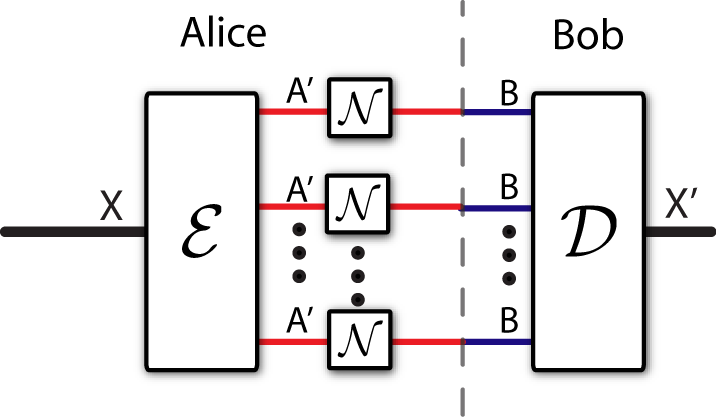
\includegraphics[width=4.8in]{mark_diagrams/quantumCapacity.png}
	
}


\frame{
	\frametitle{Encoding}
	
	We can use a quantum channel to send either classical or quantum data.


	For classical data, the encoding operation will be $\E \colon \mcal{X} \to \mcal{H}^A$,
	\be
		\E(x) = \ket{\sigma_x}^A
	\ee
	where $\ket{\sigma}_x$ is some predetermined set of ``signal states'' that will be send over the channel.
	
	
	To encode some quantum data $\rho$ we can do any quantum operation $\E \colon \mcal{H}^S \to \mcal{H}^A$,
	\be
		\E(\rho^S) = \sigma^A.
	\ee

}


\frame{
	\frametitle{Decoding classical data}
	
%			 Measurements are type of quantum operation:
%			\be
%				\mcal{M}\colon \c^2 \to (\c^2,\NN),
%			\ee
			We want to extract the classical message from the received quantum state.
			
			Measurements  act on density matrices to produce a classical 
			output as well as a possibly modified quantum state. \\
			
			Measurements are sets of projection operators $\{M_i\}$. %, s.t. $\sum_i M_i^\dag M_i = I$.
		
			The probability of outcome $m$ occurring when the input system is $\rho$ is
			\be
				p(m)	=	\Tr\!\left( M_m^\dag \rho M_m \right). \nonumber
			\ee
			
			Our example from earlier
			{\footnotesize
			\be \nonumber
			\Pr\{ \text{measure}\   x = 0\}  = \Tr \left(  
				\left[ \begin{array}{cc} 1&0 \\  0 &0 \end{array} \right]
				\left[ \begin{array}{cc} |\alpha|^2 & \beta^*\alpha \\  \alpha^*\beta &|\beta|^2 \end{array} \right]
				\left[ \begin{array}{cc} 1&0 \\  0 &0 \end{array} \right]
				\right) = |\alpha|^2
			\ee
			}
			
			%Measurements are our only way learning about quantum states. \\
			
%			The output quantum state associated with this outcome is
%			\be
%				 \hat{\rho}_m	=  \frac{M_m^\dag \rho M_m}{	\Tr\!\left( M_m^\dag \rho M_m \right)	}.
%			\ee

}


\frame{
	\frametitle{Decoding quantum data}
	
            In the error criterion for classical information theory protocols is of the form 
            $P_e = Pr\{ M_1 \neq \hat{M}_1 \}$.
            We need an analogous criterion for quantum protocols.

			The fidelity between two pure  quantum states is the square of their inner product
			\be
				F(\ket{\varphi}, \ket{\psi}) = \left\vert \braket{\varphi}{\psi} \right\vert^2.
			\ee
			
		    Two states that are very similar have fidelity close to 1. \\
		    Success criterion is
		    \be
		    	F(\ket{M}, \ket{\hat{M}}) \geq 1 - \epsilon.
		    \ee
	
}

%%%%%%%%%%%%
%%%%%%%%%%%% SURVERY OF RESULTS IN QUANTUM INFORMATION 
%%%%%%%%%%%%		
	%
	%\frame{
	%	\frametitle{quantum information theory}
	%	\begin{itemize}
	%		\item Can you do cool tricks with EPR pairs? \\
	%		$\ket{\Psi} = \frac{1}{\sqrt{2}}(\ket{00}+\ket{11})$ \\
	%		\ \\
	%		\item Can we compress quantum information? \\
	%		\ \\
	%		\item	Can you send information through a quantum channel?  \\
	%		\ \\
	%		\ \\
	%		\pause \item YES to all of the above 
	%	\end{itemize}
	%	}	

	%

	%
	%		

	%\frame{
	%		\frametitle{2$\times$ brilliant trivialities}
	%		\begin{itemize}
	%			\item 	Superdense Coding [Bennett, Wiesner 1992]:\\
	%					\be
	%						[q\,q]+[q \to q] 	\geq	2[c \to c]
	%					\ee
	%					
	%			\vspace{0.2cm}
	%			\item 	Teleportation [BBCJPW 1993]:\\
	%					\be
	%						[q\,q]+2[c \to c] \geq	[q \to q]
	%					\ee
	%					
	%		\end{itemize}
	%		}

	%

	%\frame{
	%	\frametitle{who is this?}
	%	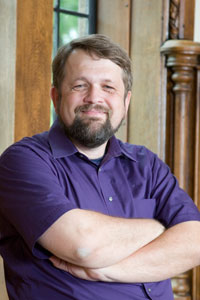
\includegraphics[width=2in]{quantum_people/SchumacherBE.jpg}

	%}

	%	
	%\frame{
	%	\frametitle{Schumacher compression}
	%	\begin{itemize}
	%	\item Start with $\rho^{\otimes n}$ ($n$ copies of state $\rho$).
	%	\item How much can you compress? \\
	%	\ \\
	%%	\item Compression rate:  
	%%		  \be
	%%		  	Q	=	\frac{strlen(compressed)}{strlen(message)}
	%%		  \ee
	%	\begin{Th}[quantum source coding]
	%		An i.i.d. quantum source $\rho$ can be compressed at
	%		a rate $R$ if $R > S(\rho)$ and cannot if $R < S(\rho)$.	\ \ \ [Schumacher 1995]
	%	\end{Th}
	%	
	%	\ \\
	%	\item How? \\
	%		  \ \ \ typical subspaces
	%	\end{itemize}
	%}

	%

	%	
	%\frame{
	%	\frametitle{quantum data compression}
	%	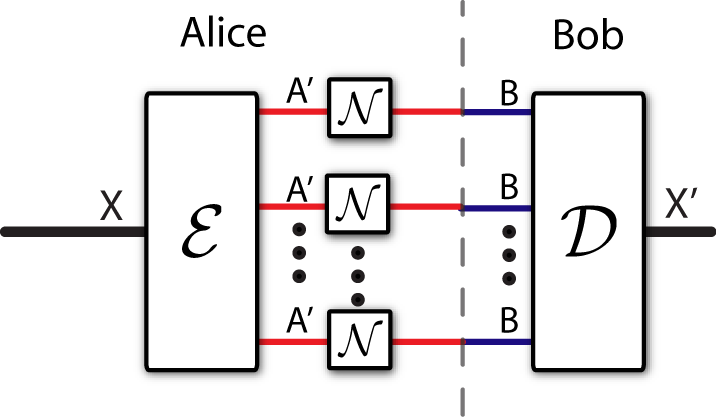
\includegraphics[width=4.8in]{mark_diagrams/quantumCapacity.png}
	%	
	%}

	%% channel capactity

	%

	%
	%\frame{
	%	\frametitle{who are these people?}
	%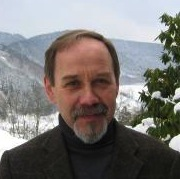
\includegraphics[height=1.6in]{quantum_people/Holevo,_Alexander2.jpg}
	%\ \ \ 
	%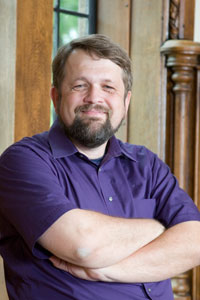
\includegraphics[height=1.6in]{quantum_people/SchumacherBE.jpg}
	%\ \ \ 
	%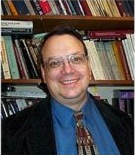
\includegraphics[height=1.6in]{quantum_people/mike_westmoreland.jpg}

	%}





%%
%\begin{frame}
%	\frametitle{Entanglement assisted}
%	\begin{itemize}
%		\item $EAC = max_\rho I(A;B) $
%		\item $EAQ = max_\rho \frac{1}{2} I(A;B) $
%	\end{itemize}
%\end{frame}



\frame{
	\frametitle{Quantum information theory}
}	



\frame{
	\frametitle{Quantum information theory}
	\begin{itemize}
	\item Came from classical information theory
	\item Replace Shannon entropy with von Neumann entropy
			\begin{Def}[von Neumann Entropy] A quantum system described by the density matrix $\rho$ has von Neumann 
			entropy $S(\rho)$ given by the expression:
			\be
				S(\rho) = - \Tr(\rho \log\rho)
			\ee
			\end{Def}
	\ \\
	\ \\
	\item 	\texttt{from classical import mutual\_information, Fano\_inequality, random\_coding,  channel\_capacity, compression, etc.. }
	\end{itemize}
}	


\begin{frame}
	\frametitle{Classical capacity of quantum channel}

    Holevo, Schumacher and Westmoreland  found a multiletter formula
    for the classical capacity  [H98,SW97].

	\begin{Th}
		The classical capacity of a quantum channel $\mcal{N}$ is
		given by  $\mcal{C}(\mcal{N}) = \frac{1}{n} \cup_{n=1}^\infty C^{(1)}(\mcal{N}^{\otimes n})$ 
		where 
		\be
	       		C^{(1)}(\mcal{N}) = \max_\rho I(A;B) 
	    	\ee
		where $\rho$ is the output state 
		    \be
		        \rho = \sum_x p(x) \ketbra{x}_A \otimes \mcal{N}\!({\sigma_x})_B.
		    \ee
		    and $\{ p(x), \sigma_x\}$ is the input distribution.
	    \end{Th}

\end{frame}



%\begin{frame}
%	\frametitle{quantum capacity}
%    Lloyd, Shor and Devetak independently proved a formula for the quantum capacity
%    of a channels.
%    
%    \begin{Th}[LSD Theorem]
%    
%    Consider the input state $\rho^{AA'}$, half of which is sent
%    through the channel $\mcal{N}$ to obtain $w^{AB} = \mcal{N}^{A'\to B}(\rho^{AA'})$.
%    Define the quantity 
%    \be
%        Q^{(1)}(\mcal{N}) = \max_\rho  (S(B)_w - S(AB)_w).
%    \ee
%    The quantum capacity $Q$ of the channel $\mcal{N}$ is given by the regularization 
%    of the $Q^{(1)}$ quantity
%    \be
%        Q(\mcal{N}) = \lim_{n\to \infty} \frac{Q^{(1)}(\mcal{N}^{\otimes n} )}{n}.
%    \ee 
%    [L97, S00, D03]
%    \end{Th}

%\end{frame}


\begin{frame}
	\frametitle{Limitations of these results}
	Not single letter ... 
         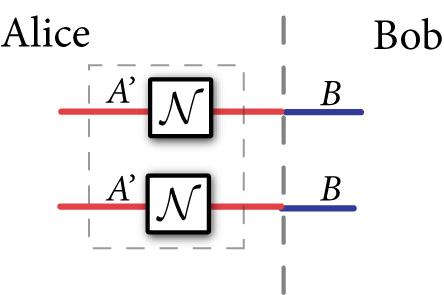
\includegraphics[height=1.6in]{mark_diagrams/notSingleLetter.png}
\end{frame}



\begin{frame}
	\frametitle{Quantum multiple access channel}

		\begin{Def} The quantum multiple access channel (QMAC) is a map
		\be
			\mcal{M}^{A'B' \to C}
		\ee
		where systems $A'$ and $B'$ are the inputs and $C$ is the output.
		\end{Def}    
		\ \\
		Three different capacities
		\begin{itemize}
			\item $\mcal{C}$: classical info
			\item $\mcal{Q}$: quantum info
			\item $\mcal{C}_E$  or $\mcal{Q}_E$: with additional resource \emph{entanglement}
		\end{itemize}
		
		
\end{frame}


\begin{frame}
	\frametitle{Classical capacity of QMAC }

		\begin{Th}[Winter 01]
		The capacity of the quantum MAC $\mcal{M}$ to carry classical information is 
		$\mcal{C}_{QMAC}(\mcal{M}) = \frac{1}{n} \cup_{n=1}^\infty \mcal{C}^{(1)}_{QMAC}(\mcal{M}^{\otimes n})$ where 
	        \be
	        		\mcal{C}^{(1)}_{QMAC}  = \operatorname{conv} \cup_{p(x_1)p(x_2)\sigma_x} \{ (R_1,R_2) | \text{ Eqn. \eqref{Gmac1} } \}  \label{region:G_MAC1}
	        \ee
	        \bea
	            R_1         &\leq&      I(A;C|B)_\theta, \nonumber \\
	            R_2         &\leq&      I(B;C|A)_\theta, \label{Gmac1} \\
	            R_1 +R_2    &\leq&      I(AB;C)_\theta, \nonumber
	        \eea 
	        where mutual informations are calculated with respect to 
		\be
			\theta = \sum_x p(x_1)p(x_2) \ketbra{x_1}_A \otimes \ketbra{x_2}_B \otimes \mcal{M}\!({\sigma_{x_1}} \otimes \sigma_{x_2} )_C.
		\ee
		\end{Th}    
		
\end{frame}


%
%\begin{frame}
%	\frametitle{Entanglement assisted capacity of QMAC}

%		\begin{Th}[Hsieh, Devetak, Winter 05]
%		The capacity of the quantum MAC $\mcal{M}$ to carry classical 
%		information \emph{when an additional resource of entanglement is available is} 
%	        \be
%	        		\mcal{C}_{E}  = \operatorname{conv} \cup_{p(x_1)p(x_2)\sigma_x} \{ (R_1,R_2) | \text{ Eqn. \eqref{Gmac1} } \}  \label{region:G_MAC1}
%	        \ee
%	        \bea
%	            R_1         &\leq&      I(A;C|B)_\theta, \nonumber \\
%	            R_2         &\leq&      I(B;C|A)_\theta, \label{Gmac1} \\
%	            R_1 +R_2    &\leq&      I(AB;C)_\theta, \nonumber
%	        \eea 
%	        where mutual informations are calculated with respect to 
%		\be
%			WRONG
%			\theta = \sum_x p(x_1)p(x_2) \ketbra{x_1}_A \otimes \ketbra{x_2}_B \otimes \mcal{M}\!({\sigma_x})_C.
%		\ee
%		\end{Th}    
%		
%\end{frame}





\begin{frame}
	\frametitle{Quantum interference channel}
    
	
	\begin{Def}
		The quantum interference channel is a map
		\be
			 \mathcal{N}^{A_{1}^{\prime}A_{2}^{\prime}\rightarrow B_{1}B_{2}}
		\ee	
	
	\end{Def}
	
	
    	Open problem. \\


	can adapt some of the classical results...
	
\end{frame}



\begin{frame}
	\frametitle{Entanglement assisted}
	\begin{center}
         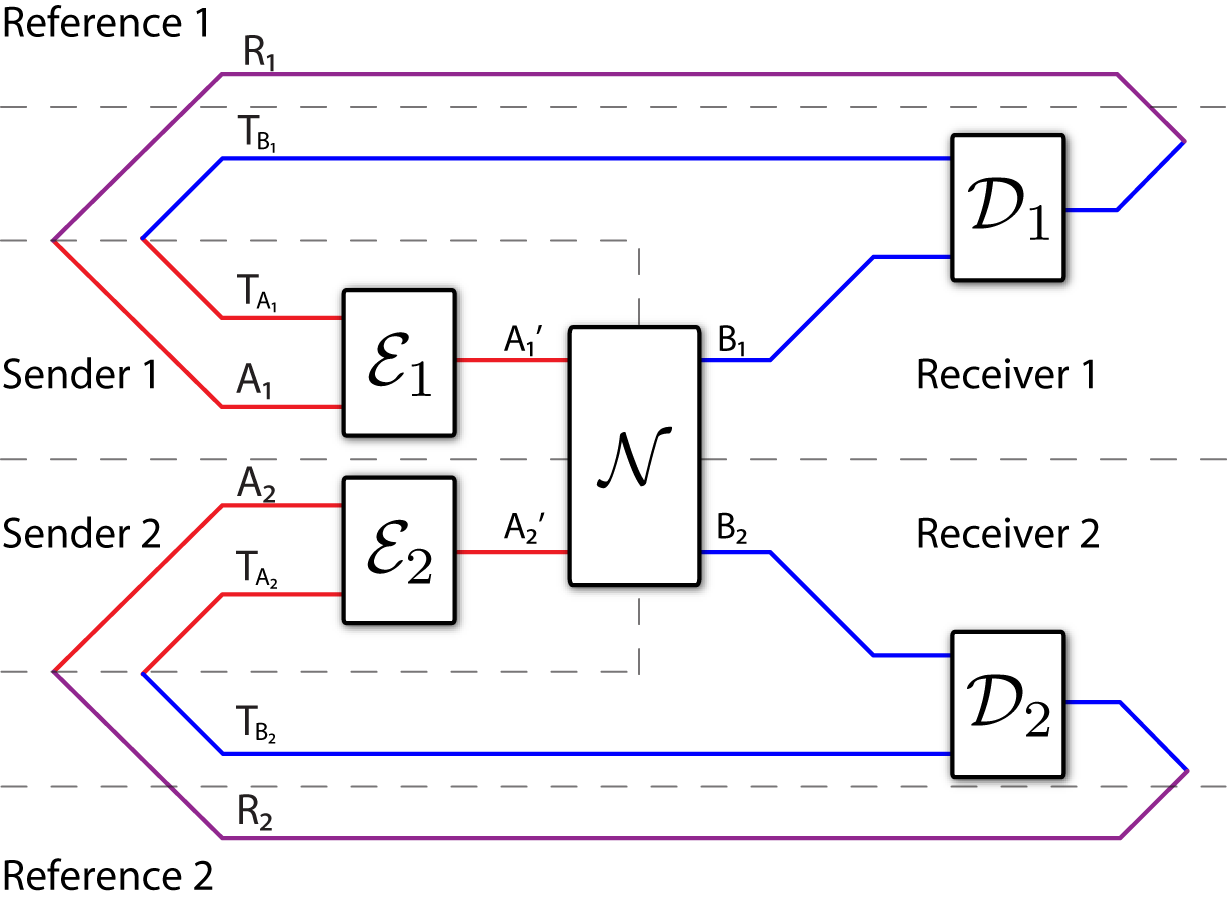
\includegraphics[height=2.7in]{mark_diagrams/interference-protocol.png}
	\end{center}
\end{frame}










\begin{frame}
	\frametitle{The end}
	\begin{center}
		\huge thanks for your attention!
	\end{center}
\end{frame}



\frame{
	\frametitle{Physicist's view}
	
        \begin{itemize}
%        	\item QM is useful
	\item Very similar to what we learn in signals and systems
	
	\pause
	\item	 A quantum state (signal) is represented by a  \emph{wavefunction} 
		\be
			%i am not sure if I can handle this...
			%\psi \colon \mathbb{R}^3\times t \to \mathbb{C} 
			% so lets skip time... say it is an open problem...
			\psi \colon \mathbb{R}^3 \to \mathbb{C} 
		\ee

	\item	  	The wave function of Hydrogen's ground state (n=1 $\ell$=0) 
			\be
				 \psi(r,\vartheta,\varphi) =  \sqrt{	  \frac{1}{\pi a^3}   }  \exp\left(\frac{- r}{ a} \right),
			\ee
			in the \emph{position} basis. Apply Fourier transform to get \\ the \emph{momentum} basis
	
        %The continuous \emph{wavefunction representaiton} of quantum mechanics is useful in optics,
        %atomic physics and solid state physics, where people calculate things by integrals in 
        %the position basis (Diract $\delta(x)$ functions),
        %and its fourier transform ($sin(\omega x),cos(\omega x)$) the momentum basis.


	\end{itemize}
}

\frame{ 
	\frametitle{Physicist's view (continued)}
	
	\begin{itemize}
	\item 	The power of the signal is a probability density\
			\be
				\Pr\{ \text{finding electron at} \ \ \vec{r} \ \} =  |\psi(\vec{r})|^2 
			\ee
	\item 	Verify that it is well normalized
			\bea P_{total} &=& \int\!\!\int\!\!\int |\psi(\vec{r})|^2  \  d^3\vec{r} \nonumber \\
				 &=& \int_0^\infty\int_0^{2\pi}\int_0^\pi  |\psi(r,\vartheta,\varphi)|^2  \ r^2 \  \sin \varphi d\varphi d\vartheta dr   \nonumber  \\
				 &=& \int_0^\infty \frac{4}{a^3} \exp\left(\frac{2 r}{a}\right) r^2 \ dr  =  1 
				%		\int_0^\infty \frac{4}{a^3} \exp\left(\frac{2 r}{a}\right) r^2 \ dr = 1  \text{if}   \Re(a)>0
			\eea
	\end{itemize}		
	
}



\end{document}
